\chapter{插图的使用演示}

\label{chap:figure}
\section{插图的演示}

插图建议在figures目录中设置对应的tex文件。比如,我们在figures/chapter2/linear.tex文件中定义了图像,并把原图像放置在images目录中,在需要时使用如下命令插入图像:
\begin{verbatim}
\begin{figure}[htb]
    \centering
    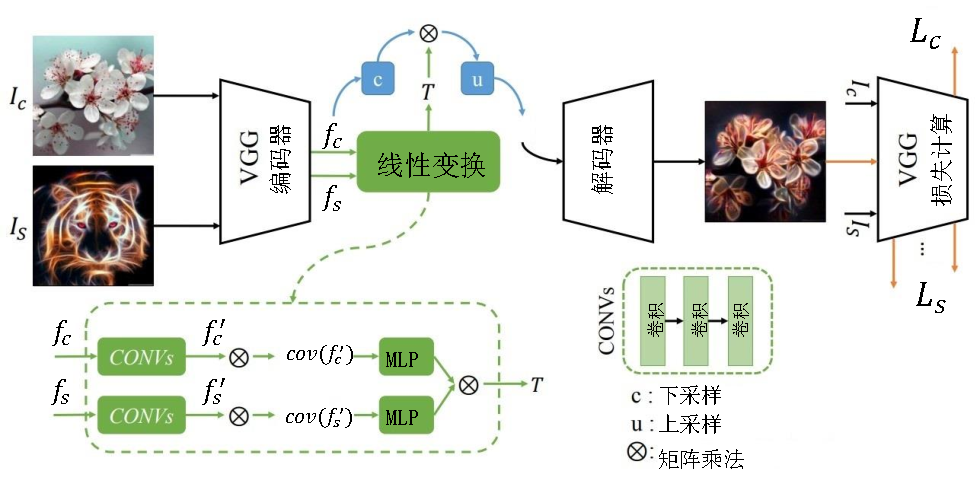
\includegraphics[width=.8\linewidth]{images/chapter2/linear.pdf}
    \caption[基于线性变换的图像风格化网络结构示意图]{基于线性变换的图像风格化网络结构示意图~\cite{Li_2019_CVPR}}
    \label{fig:linear}
\end{figure}
\end{verbatim}
上面命令的作用就插入了如下图像:
\begin{figure}[htb]
    \centering
    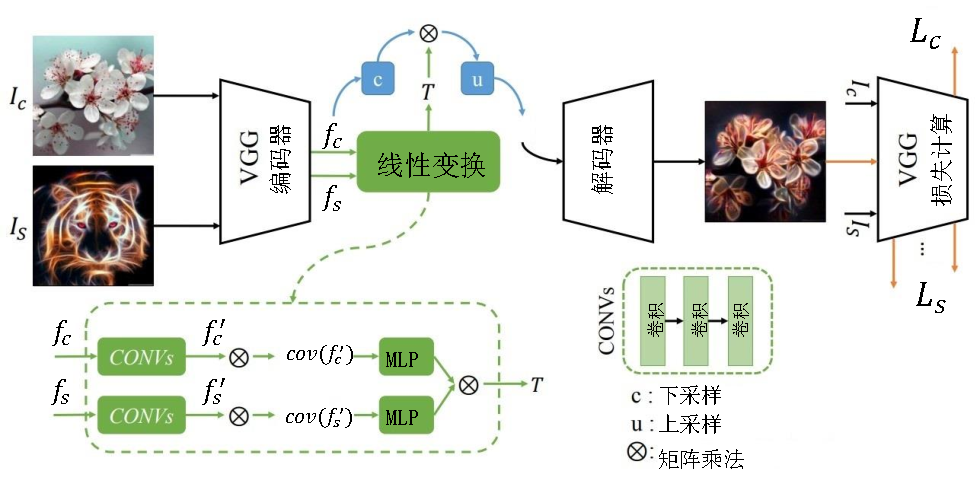
\includegraphics[width=.8\linewidth]{images/chapter2/linear.pdf}
    \caption[基于线性变换的图像风格化网络结构示意图]{基于线性变换的图像风格化网络结构示意图~\cite{Li_2019_CVPR}}
    \label{fig:linear}
\end{figure}

当然,在正文中也是可以根据自己设置的label来引用的图像的,比如用
\begin{verbatim}
\cref{fig:linear}
\end{verbatim}
这一命令来引用自定义的label。效果如下:

Li等人~\cite{Li_2019_CVPR}提出了一种基于线性变换的任意风格化方法。
完整的基于线性变换的任意风格化方法如\cref{fig:linear}所示。

你可以注意到,在图像的caption中,
\begin{verbatim}
    \caption[基于线性变换的图像风格化网络结构示意图]{基于线性变换的图像风格化网络结构示意图~\cite{Li_2019_CVPR}}
\end{verbatim}
被[]包裹的是在目录中显示的内容,被\{\}包裹的是真正在caption显示的内容。同时,caption内是可以添加文章的引用的。